\chapter{Results and Considerations}
In this chapter there will be discussed the results and the material created during all the work of this thesis.\\

It is important to say that the results are not the only parameter defining if a good verification work was done or not. In fact building the infrastructure and create documentation are important tasks that every verification engineer will eventually do, and they will produce results in long term, so it could be possible they are not directly correlated to some found bug.\\


\section{Found Bugs}
The thesis was developed while the design was on going and so unstable. To synchronize all the work it was used the GitLab structure, creating issues and discussing the problems. A well defined issue was then assigned to a design engineer to fix it.\\

The majority of the bugs were found on the Load Management Unit. Let's now analyze some of them.\\

\subsubsection{the indexed load bug}
This one is an issue found using the Formal tools and trying to define better specifications for the Load Management Unit.\\

The problem was the following:
The LMU used the sequence\+id, in particular the \emph{el\+count} field, to identify if the load was strided or indexed. In particular, el\+count contains the number of valid elements being loaded; when this value was el\+count = 1 then the load was considered as indexed.\\
The issue was presenting because the indexed load should ignore the stride value, and so there is no way to send only one element with a stride, or better, in this case the load would not ignore the stride, as every operation was actually a strided one.\\

The better solution for this problem was to create a new signal, \emph{is\+indexed}, to identify an indexed load. The stride will be always ignored when this signal is asserted, and the value of el\+count must be = 1.\\

\subsubsection{the out-of-order load bug}
This issue regards the out-of-order loads. In the Load Management Unit there is a FIFO handling the load\+ids for the two possible inflight loads.\\

The FIFO was freed of an element only when another one was put as input. But it could have been possible that an already inflight load was into the FIFO, let's say with id = 1, and another load with id = 1 issued. \\
Having the same id the configurations for the second load would have been overwritten.\\

This issue was found analyzing the result of two consecutive loads, with same id, but one was strided and another one was indexed. The second load was not considered as indexed failing the condition that says el\+count = 1.\\

This was the case of a typical bug finding flow: first the whole big tests fails during a load. Then it is examined using the assertions on the load modules. Exploring the waveform is then possible to find the bug.\\

\subsubsection{the after kill bug}
This bug is related to the validity of the data in output to the LMU.\\

When there is a kill, the entire instruction needs to be killed. But it could be possible to receive valid data for a killed load. This because the kill needs some time to stop the operation.\\

So the LMU should ignore the input from a killed instruction, but this was not the case. Indeed the validity of the data in output was assumed every time the data was valid in input.\\

It caused the simulation to time out on the next instruction. This because the kill was not issue correctly, so the starting point for the next instruction was not clean. \\

This issue can represent a valid example of why the formality on the assertions in very important.\\
Consider the following code:\\

\linespread{1}
\begin{lstlisting}[language=Verilog,style=verilog-style, backgroundcolor=\color{lyel_palette}, frame=tlb]
property p_dvalid_o;
@(posedge clk_i)
load_data_valid_i && sb_correct |-> ##1 load_dvalid_o ;
	endproperty : p_dvalid_o

a_dvalid_o : assert property( disable iff(!rsn_i || kill_i) p_dvalid_o )
else $error('LMU did not compute any output');
\end{lstlisting}
\linespread{1.2}

In this case, the assertion is testing if there is \emph{load\+dvalid\+o} when the input is valid. But it does not test if \emph{load\+dvalid\+o} has always a valid \emph{load\+data\+valid\+i} a clock cycle before.\\

The property as reported is not able to spot the error in this issue, but knowing where is the problem is possible to use the correctness of this assertion to understand the problem.\\

\subsubsection{the two loads bug}
This issue was spotted both in the LMU and in the LB. The modules received two loads with the same id. This led to an assumption error, as every load has an unique id.\\

In reality the problem was not in the Load Management Unit nor in the Load Buffer, but in the memory queue. In fact, this modules is the responsible to hand the ids for each load.\\

Also this issue was found so late in the verification process because was depending on a trigger enabled by the kill.\\

For reference in Figure \ref{2-loads} there is the interface of a simulation, in particular on the waveforms. It is possible to see two loads issue with the same id.\\

\begin{figure}[H]
    \centering
    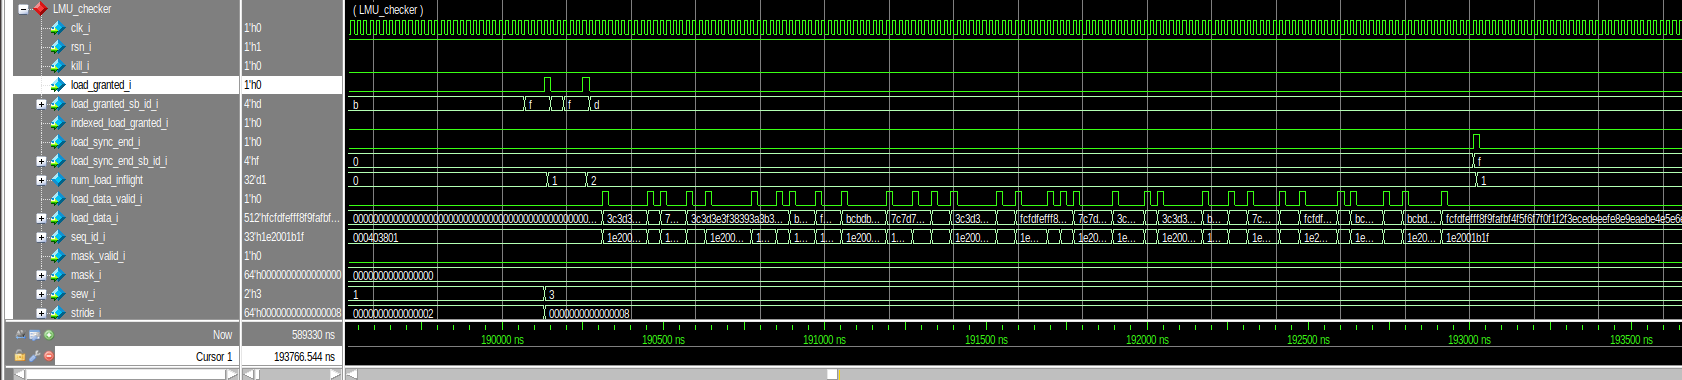
\includegraphics[scale = 0.25]{Chapter_3/img/2-loads.png}
    \caption{Two loads issued with ther same id}
    \label{2-loads}
\end{figure}

\section{Material Created}
Other than the founded bugs there is also some material created during this thesis.\\
In particular on the structure to handle the test of the submodules.\\

\subsubsection{UVM}
A complete UVM was created, to drive and test the Load Management Unit. It has also the possibility to have different tests with different sequences and so constraints.\\

\linespread{1}
\begin{lstlisting}[language=Verilog,style=verilog-style, backgroundcolor=\color{lyel_palette}, frame=tlb]
class lmu_constrained_test extends lmu_random_test;
    `uvm_component_utils(load_management_unit_constrained_test)

	function void build_phase(uvm_phase phase);
		lmu_sequence_item::type_id::
		  set_type_override(lmu_constrained_sequence_item::get_type());
		super.build_phase(phase);
	endfunction


	function new(string name, uvm_component parent);
      		super.new(name,parent);
   	endfunction : new


endclass : lmu_constrained_test
\end{lstlisting}
\linespread{1.2}
In this code the base\+test is extended and then it is overridden into the build\+phase the sequence\+item.\\
\linespread{1}
\begin{lstlisting}[language=Verilog,style=verilog-style, backgroundcolor=\color{lyel_palette}, frame=tlb]
class lmu_constrained_sequence_item extends lmu_sequence_item;
	`uvm_object_utils(lmu_constrained_sequence_item)

	constraint few_rst{op dist{rsn_op:=1,gnt_op:=5,load_op:=9,kill_op:=2};}
	

	function new(string name = "");
		super.new(name);
	endfunction : new

endclass : lmu_constrained_sequence_item
\end{lstlisting}
\linespread{1.2}
In the sequence new constraints are applied. In this case the probability for the operation are defined.\\

This kind of structure is very reusable and expandable, also and it can be improved during the whole verification process.\\

\subsubsection{specifications}
Other than that some documentation was created, on missing specifications and on guides to perform certain kinds of checks. This is very important during a project because allows the other members to partecipate actively.\\

This work was not done in one shot, but required a looped check on the behaviour obtained. The specs and the design were still being developed, this means also the documentation should have been. But this was not always the case, so a constant check (helped also with the formal tool, very useful to define the correct assumptions) helped maintain the documentation correct.\\

\subsubsection{verification plan}
The verification plan was half prepared when the work of this thesis started. However when starting the creation of the checkers a lot of changes were upcoming, so important modifications were done to the test plan. It was also done following a standard to avoid incompatibilities when using it with other software.\\
The assertion reported into the Appendix are following the verification plan implemented.\\

\subsubsection{test plan}
The test plan for the loads was entirely created during the process of this thesis. It required first some confidence with the load operation, then it was possible to update the simple cases and fill it with interesting corner cases.\\

In order to give validity to the test plan it was important to create an easy way to run those tests. For that were done some configurable modalities.\\


\subsubsection{modalities}
The last contribute was to create the modalities for the implemented tests. In the code below it is possible to see a couple of them.\\

\linespread{1}
\begin{lstlisting}[language=Verilog,style=verilog-style, backgroundcolor=\color{lyel_palette}, frame=tlb]
//(for beautiness there is also a subtraction in case of overflow, 
//in order to start from the smallest index possible).
//The range_id is NOT getting smaller as the overflow occurs, 
//because we do not want to cause more retries, so we put the index fixed to 0

else if (m_cfg.seq_id_mode == RETRY_ID) begin
    if(loop_ooo[load_index] <= 3 & loop_ooo[load_index] > 0) begin
        range_id[load_index] = c_lines_per_group -1 ;
        seq_id_index[load_index] = (seq_id_index[load_index] +
            range_id[load_index])%(inflight_loads[load_index].seq_ids.size());
            
    end
    else seq_id_index[load_index] = 0;
        loop_ooo[load_index] += 1;
        
end


//Here we want to stimulate 0-40-120-80 id seq, 
//so we choose the correct cycle value and manipulated the range.
//then the cycle after the range returns to be 4 and stale.

else if (m_cfg.seq_id_mode == RETRY_OOO_ID) begin
    if(loop_ooo[load_index] == 0) begin
        range_ooo_id[load_index] = c_lines_per_group - 1;
        seq_id_index[load_index] = 0;

    end else begin
        if(loop_ooo[load_index] == 3) 
            range_ooo_id[load_index] = 2*range_ooo_id[load_index] + 1;
        if(loop_ooo[load_index] == 4) 
            range_ooo_id[load_index] = -(c_lines_per_group);
        if(loop_ooo[load_index] == 5) 
            range_ooo_id[load_index] = c_lines_per_group -1;
        seq_id_index[load_index] = (seq_id_index[load_index] +
            range_ooo_id[load_index])%(inflight_loads[load_index].seq_ids.size());
        if(loop_ooo[load_index] > 5) 
            seq_id_index[load_index] = 0;
    end
    loop_ooo[load_index] += 1;
end



\end{lstlisting}
\linespread{1.2}

It is possible to see the handling of the element id sent by avispado. In this case it is manipulated the order of the ids, and this will not cause an error as the final result will be the same.\\

In this way it is possible to stimulate the retry mechanism sending all the elements for the same position into the Load Buffer. There is also another version for the out-of-order retry.\\

Those modalities can be configured for each test, and so randomized. In this way they can be implemented in the automatic tests.
